%3章
\chapter{提案手法}

本研究で対象とするエージェントシミュレーションの大きな特徴は,介護の対象となる高齢者の運動機能や認知機能の低下に大きなバリエーションがあると同時にも,介護者側にも国家資格をもった介護福祉士から,介護ヘルパー,ボランチィアスタッフまで技能や知識,経験に大きなバリエーションがあることである.そうしたことを念頭に置いた上で,本研究では介護者エージェント,被介護エージェント,環境としての高齢者施設の基本モデリングを検討した.図\ref{concept_simulation}に概念図を示す.黒で示される介護者が,自身が持つ視野の中で水色で示される被介護者を観測する.

\begin{figure}[htb]
\begin{center}
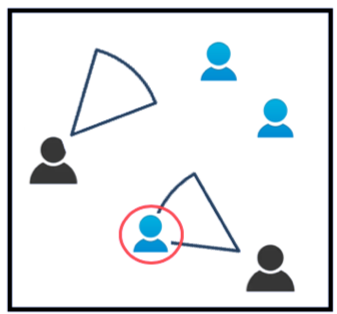
\includegraphics[scale=1.4]{figures/concept_simulation.png}
\caption[シミュレーションの概念図]{シミュレーションの概念図 \label{concept_simulation}}
\end{center}
\end{figure}

\section{知的マルチエージェントモデル}

介護行動は社会系の複雑現象である.私たちが行動を起こす際に,認知症による自己の生理機能への理解が周囲に与える影響を懸念することはあっても,それの繰り返しによって大きな事故につながると理解している人は少ない.しかし,個人レベルでは,手すりに捕まる,他の歩行者に接触しないようにするといった比較的単純なルールに従い行動しているが,それらの個人行動が多種・多量に存在し,相互作用することによって全体としては非常に複雑な現象となる.複雑系を解析する手法の一つとして,マルチエージェント手法がある.しばしば,セルオートマトンが複雑系のシミュレーションに用いられ,セルオートマトンに基づくシミュレーションの研究事例もいくつか存在する.これに対して,本シミュレータでは,人間という知的レベルの高い主体が多数集まり相互作用を起こす介護現象をより精緻に再現するために,情報を知覚し,それを基に自律的に行動を起こす主体を知的エージェント,それを取り巻く世界を環境と定義し,シミュレーションの構造はマルチエージェントのフレームワークに基づき構築している.そこで,これを知的マルチエージェントモデルと呼ぶ.

\subsection{知的エージェントの構築}
図\ref{intelligent_agent}に知的工一ジェントのイメージを示す.知的エージェントは,情報を知覚するセンサーと動作を実行する作用器を持っている.また,エージェント自身の思考プロセスを保持しており,センサーから得られた情報と自分の有する知識と判断基準に基づき自律的に行動を決定し,作用器を通して行動を起こし,環境に働きかける.センサー,作用器,思考は知的エージェントが実際に適用される時点で,問題に応じて定義される.図\ref{agent_modeling}にエージェントと環境の相互作用の様子を模式的に示す.介護者エージェントが自らの行動により環境に影響を与え,その環境によって被介護者エージェントが影響を受けることになる.ある主体の動きによって系全体の動きが規程され,複雑な現象が創発する.

\begin{figure}[htb]
\begin{center}
 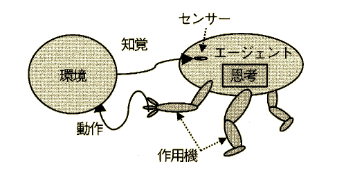
\includegraphics[scale=0.8]{figures/intelligent_agent.png}
 \caption[知的エージェントの模式図]{知的エージェントの模式図 \label{intelligent_agent}}
\end{center}
\end{figure}

\begin{figure}[htb]
\begin{center}
 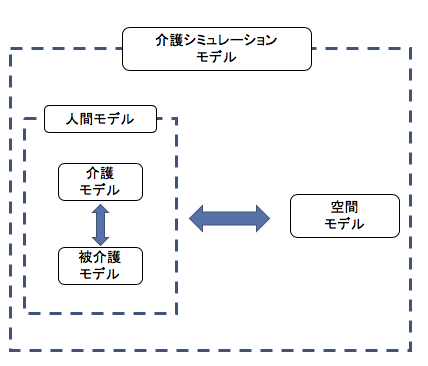
\includegraphics[scale=0.6]{figures/agent_modeling.png}
 \caption[本シミュレーションにおける環境とエージェント]{本シミュレーションにおける環境とエージェント \label{agent_modeling}}
\end{center}
\end{figure}

\subsection{シミュレーションフロー}

本研究におけるシミュレーションの流れの概略図を図\ref{simulation_flow}に示す.まず,高齢者施設,介護者,被介護者といった空間を構成する要素を環境として構成し,その後実際にシミュレーションを開始する.タイムステップごとに,各エージェントの内部状態を変化させ,介護シミュレーションを行っていく.被介護者の場合は,時間経過で尿量を加算し,エージェントごとに設定されている閾値を超えた時点で介護アラートを出す.介護者は,自分の周りで介護アラートが出たタイミングで,自らと最も距離の近い被介護者のもとへの介護に向かう.これを繰り返すことがシミュレーションが進んで行く.

\begin{figure}[htb]
\begin{center}
 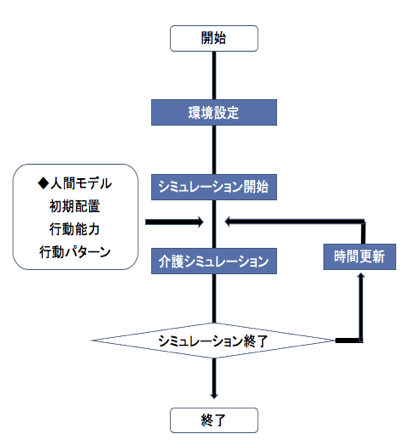
\includegraphics[scale=0.6]{figures/simulation_flow.png}
 \caption[シミュレーションフロー]{シミュレーションフロー \label{simulation_flow}}
\end{center}
\end{figure}

\section{仮想環境}
本シミュレータにおける環境とは,高齢者施設とそこに存在する介護者,被介護者構造を指す.高齢者施設のモデル化はそれ自体が交通流シミュレータの汎用性・拡張性を実現する上で重要な課題である.本シミュレータでは,介護者・被介護者は基本的に.自由移動を行うことができる二次元平面を想定している.

\subsection{高齢者施設}

今回の開発では,高齢者施設を表現するための第1ステップとして,Social Force Modelを利用するため自由に歩行できる連続空間を対象とし,壁に囲まれた移動可能な二次元平面を作成した.高齢者施設をもした空間を作成するために,$x$座標,$y$座標を持つ壁を構築した.壁は中心の座標と,壁の幅として$dx$,$dy$をそれぞれの方向に持つ.また,壁の向きを$\theta$として定義し,どの方向にも回転できるようにしている.

\subsection{Vectorモデル}

本シミュレーションにおいては,1次元での移動のみだけでなく,2次元方向での移動を考慮するために,新たなベクトル演算のクラスを実装し,Vector2Dクラスとした.Vector2Dクラスを用いて位置ベクトルや速度ベクトルをベクトル表記し,ベクトル同士の四則演算や,単位ベクトルへの変換を容易に行えるようにモデルを改良した.

\section{歩行者モデル}

本研究では,後述の介護者モデル,被介護者モデルを実装するために,それぞれの上位概念である歩行者モデルを考える.以下に歩行者モデルの実装において用いた経路選択や加速度決定の手法について述べる.

\subsection{経路決定モデル}

歩行者エージェントは出発地から目的地まで大域的な移動を行うため,歩行者の経路選択機能を実装する必要がある.経路選択機能とは,エージェントが自律的に目的地へ向かうまでの経路を選択する機能のことを指す.本研究ではエージェントには発生時に目的地が与えられるものとし,各エージェントが現在地点から目的地まで進むために,各々の行動を最適化していくことを考える.
歩行者は最短経路となる経路選択を行うという仮定に基づいて,最短経路になるように被介護者への動線,介護目的地までの動線を決定すると考える.これは,一般的な歩行者が経路選択を行う際に,多くの歩行者が,経路長が短いことを優先させようとするという習性を反映させたものである\cite{choice_route}.
この前提のもと,介護者は,初期的に与えられた目的地群の中で見回りを行い,被介護者から介護アラートを感知した時に,再度経路探索を行い,自らの目的地を再設定する.

\subsection{加速度決定モデル}

介護者,被介護者は2次元の高齢者施設に存在するため,方向と速度の制御を行わなければならない.今回は,歩行者の行動モデルとしてSocial Force Model\cite{SFM}を採用した.歩行者シミュレーションの研究分野においては,様々なモデル化が検討されている\cite{ex_pedestrian_simulation_1,ex_pedestrian_simulation_2}.たとえば,磁気モデルを用いると多方向に歩行するエージェントの相互作用を効率的に記述することが可能である.しかし,今回の研究のように閉二次元平面での歩行を対象とする場合には,部屋の中を目的地に対してどう動いて行くかを単純に記述するモデルで十分である.また歩行者モデルとしてあまり複雑なモデルを採用すると計算量が増大しシミュレータの大規模化が困難であることがSocial Force Modelを採用した理由である.

Social Force Modelは,歩行者を2次元の粒子であると仮定し,その粒子に以下の4つの力が働くと仮定するモデルであるが,介護施設の中でそれら力が具体的にどのような時に生じるかを説明する.

\begin{itemize}
 \item 移動目標に近づく力
 \item 他のエージェントからの斥力
 \item 壁などの環境からの斥力
 \item 魅力的な環境への引力
\end{itemize}

移動目標に近づく引力は,エージェントが当初想定していたコースからはずれてしまった場合に目的地の進行方向へと曲げるように働く力のことであり,他のエージェントや壁などからの斥力は,エージェント間,あるいは壁とエージェント間との距離を考える.本研究では,介護者と被介護者は必要があればお互いが近く関係にあるので,これら斥力は被介護者同士でのみ発生することとなる.魅力的な環境への引力では,高齢者支援施設の中では手すりのような,歩行者にとって近づくことのインセンティブが発生するようなものへの引力のことである.

\subsection{介護者エージェント}

介護者エージェントは上述の歩行者としての基本的な能力を備えつつ,さらに自らの介護能力と,介護可能かどうかの介護ステータス,さらにどの被介護者を優先的に介護すべきかという事前情報を実装する.

\subsubsection{介護プロフェッショナル段位制度}

介護能力を実装するために,介護プロッフェッショナル段位制度\cite{kentoukai}をもとにする.第1回介護プロフェッショナルキャリア段位制度の在り方に関する検討会資料によると,図\ref{kaigo_professional}のように介護者のレベルが設定されている.

\begin{figure}[htb]
 \begin{center}
 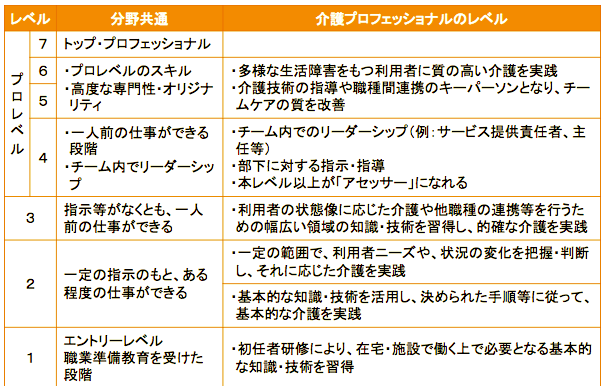
\includegraphics[scale=0.4]{figures/kaigo_professional.png}
 \caption[介護プロフェッショナル制度による介護レベル]{介護プロフェッショナル制度による介護レベル \label{kaigo_professional}}
 \end{center}
\end{figure}

これを元に,介護レベルを設定する.ある被介護者が介護アラートを出した時に,一人で介護を行うことができる介護者と,自分を含め他の介護者に指示を出すことのできる介護者,指示されなければ介護を行うことができない介護者のように介護者の介護能力によってバリエーションを設ける.

\begin{figure}[htb]
 \begin{center}
 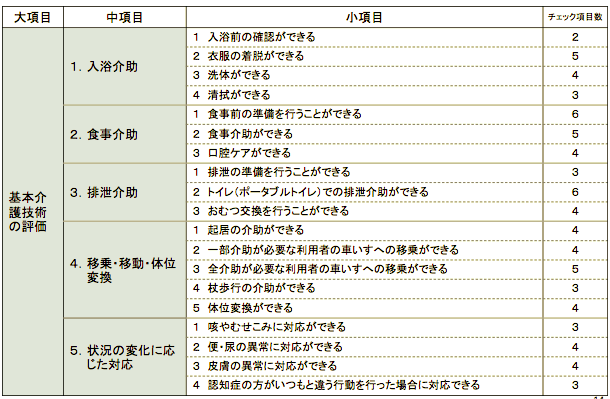
\includegraphics[scale=0.4]{figures/practical_skill}
 \caption[実践的スキルのチェック項目]{実践的スキルのチェック項目 \label{practical_skill}}
 \end{center}
\end{figure}

さらにこの検討会では,図\ref{practical_skill}に示した通り,実践的スキルについてより詳細に評価されており,これらを用いることで,介護アラートの種類を複雑化していく中でも,より適切に実際の看護現場を再現することができる.

\subsubsection{介護ステータス}

介護ステータスとして,介護可能かどうかを判定する機能を実装する.介護中の場合は,他の被介護者が介護アラートを出した場合でも対応することができない,あるいは他の介護者に役割を任せ,新たに経路探索をし直す必要があるために,そのような状況にも対応できるように,同じ介護者でも複数パターンの対応を行うために介護ステータスを実装した.

\subsection{被介護者エージェント}

被介護者エージェントについては,介護者エージェントと同様にSocial Force Modelを軸に,歩行者エージェントを作成し,それに加えてエージェントの状態によって時系列的に発生する要介護行動を実装した.高齢者の排尿に関する実態研究\cite{micturition}によると,排尿障害症状を自覚している人は男子が38%,女子が23%と高い水準にあり,男子では排尿困難症状が多く,女子では頻尿を訴える例が多かった.また明らかな尿失禁を抱えているのにも関わらず,その存在を知られたくないという心理が半数以上の人に認められたことも挙げられている.これらから,実際にトイレに行きたいと思っているかどうかの認知についてと,トイレで正常に排尿を行えるのかどうかといった機能について,被介護者のバリエーションを設けることとした.

\subsubsection{要介護認定}

介護者が事前情報として,どの被介護者から介護すべきかと言うことを判断する基準の一つとして要介護度が存在する.要介護認定は,介護サービスの必要度(どれ位,介護のサービスを行う必要があるか)を判断するものです.要介護認定 介護認定審査会委員テキスト\cite{youkaigodo}によると,基本調査において把握した申請者の「能力」,「介助の方法」,「障害や現象(行動)の有無」を調査した結果と,これらを総合化した指標である5つの中間評価項目得点を併せて「状態像」を定義している.介護サービスの必要度(どれ位,介護サービスを行う必要があるか)の判定は,図\ref{hantei}のように,客観的で公平な判定を行うため,コンピュータによる一次判定と,それを原案として保健医療福祉の学識経験者が行う二次判定の二段階で行っている.

\begin{figure}[htb]
 \begin{center}
 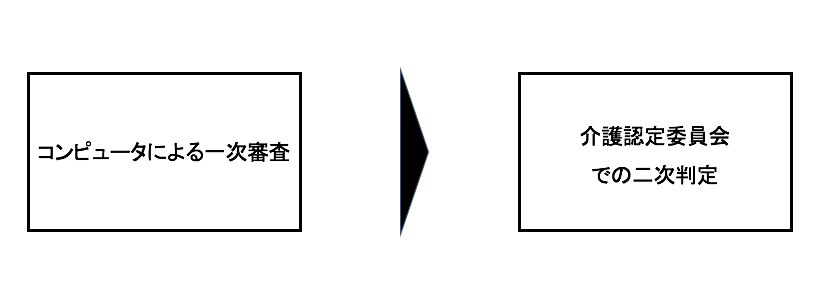
\includegraphics[scale=0.4]{figures/hantei}
 \caption[要介護認定の判定フロー]{要介護認定の判定フロー \label{hantei}}
 \end{center}
\end{figure}

一次判定のコンピュータシステムは,認定調査の項目等ごとに選択肢を設け,調査結果に従い,それぞれの高齢者を分類してゆき,「1分間タイムスタディ・データ」の中からその心身の状況が最も近い高齢者のデータを探しだして,そのデータから要介護認定等基準時間を推計するシステムです.この方法は樹形モデルと呼ばれ,その概要を\ref{tree_model}に示す.なお,1分間タイムスタディ・データとは,介護老人福祉施設や介護療養型医療施設等の施設に入所・入院されている3500人の高齢者について,48時間にわたり,どのような介護サービスがどれ位の時間にわたって行われたかを調べたものである.

\begin{figure}[htb]
 \begin{center}
 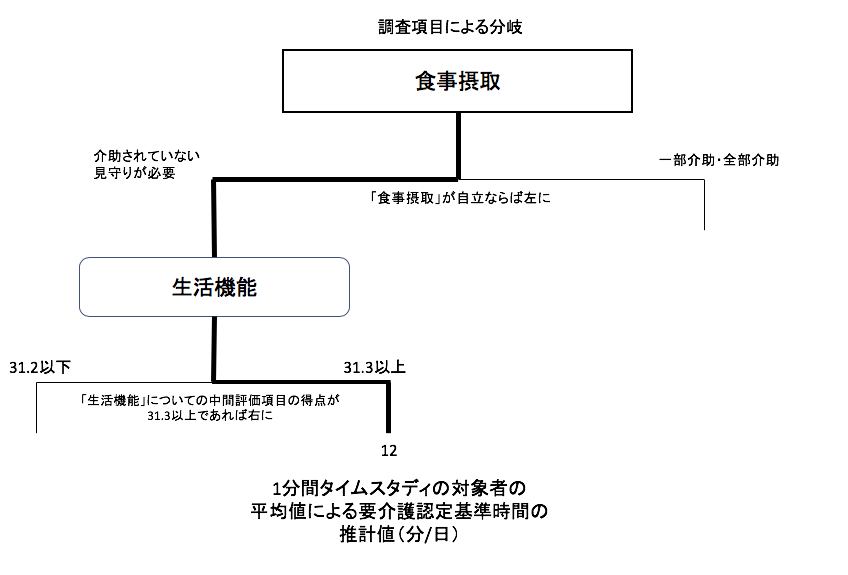
\includegraphics[scale=0.4]{figures/tree_model}
 \caption[樹形モデルの概要]{樹形モデルの概要 \label{tree_model}}
 \end{center}
\end{figure}

これを元に,5分野(直接生活介助,間接生活介助,BPSD関連行為,機能訓練関連行為,医療関連行為)について,要介護認定等基準時間を算出し,その時間と認知症加算の合計を基に,表\ref{care_level}のように要支援1から要介護5に判定される.

\begin{table}[htb]
  \caption[要介護の分類]{要介護の分類}
  \label{care_level}
  \centering
  \scalebox{0.8}{
  \begin{tabular}{r|c}
    分類 & 状態 \\ \hline
    要支援1 & 要介護認定等基準時間が25分以上32分未満又はこれに相当すると認められる状態 \\
    要支援2,要介護1 & 要介護認定等基準時間が32分以上50分未満又はこれに相当すると認められる状態 \\
    要介護2 & 要介護認定等基準時間が50分以上70分未満又はこれに相当すると認められる状態 \\
    要介護3 & 要介護認定等基準時間が70分以上90分未満又はこれに相当すると認められる状態 \\
    要介護4 & 要介護認定等基準時間が90分以上110分未満又はこれに相当すると認められる状態 \\
    要介護5 & 要介護認定等基準時間が110分以上又はこれに相当すると認められる状態 \\
  \end{tabular}
  }
\end{table}

要介護レベルのように,被介護エージェントにバリエーションをつけることができる.本シミュレーションでは,被介護エージェントにcare levelを設定し,介護者の事前情報として介護の優先順位を決定できる分類を実装した.

\subsubsection{内部変数}
被介護エージェントは内部変数として,生体情報である尿量を持っており,時間経過で尿意を催す.1日に1000から1500mlの尿を排出し,1日8から10回程度排尿するという前提のもと実装を行なった.

\subsubsection{介護アラート}

被介護エージェントはあらかじめ設定した条件を満たした時点で介護アラートを発する.本研究では,適切な尿量である100-150ml程度,膀胱に尿が溜まった時点でアラートを発する.あるいは,要介護レベルの高い被介護者が自力で歩き出した際に,転倒を想定した介護アラートのように,被介護エージェントから能動的に発するものに加えて,介護者が発見して初めて気付くものも介護アラートとする.

\subsection{介護ペア選択アルゴリズム}

上述のように,被介護者がアラートを発した時にどの介護者とマッチングさせるのかというのがシミュレーション上必要になる.本研究では,各タイムステップごとにある被介護者がアラートを出した時点で,その被介護者と介護可能な介護者との距離を計算し,ペアになりうる介護者と被介護者のペア候補配列を作成していき,その中で全探索を行うことで,最も距離の近いペアを作成して行くこととする.
